\begin{exercício}{Cascas esféricas concêntricas preenchidas por um dielétrico linear}{exercício5}
    Considere duas cascas esféricas metálicas concêntricas de raios \(a\) e \(b\), com \(a < b\). A casca de raio \(b\) está aterrada enquanto que a casca de raio \(a\) encontra-se mantida a um potencial \(\phi_0 > 0\). Na região entre as cascas há um dielétrico linear de constante dielétrica \(k\) preenchando apenas metade da região, como mostra a figura abaixo, onde \(\epsilon = k \epsilon_0\).

    \begin{center}
        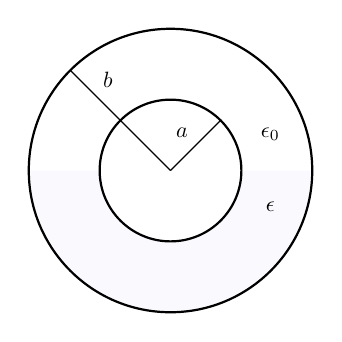
\begin{tikzpicture}[scale=0.6,every node/.style={scale=0.8}]
            \def\a{1.5}
            \def\b{3}
            \def\t{0}
            \path[fill=Lavender!20] +({180 - \t}:\b) arc[start angle={180-\t}, end angle={360+\t}, radius=\b]  -- ({\a*cos(\t)}, {\a*sin(\t)}) arc[start angle={360+\t}, end angle={180 - \t}, radius=\a] -- cycle;
            \draw[thick] (0,0) circle (\b);
            \draw[thick] (0,0) circle (\a);

            \node at +({\t + 20}:{(\a + \b)/2}) {$\epsilon_0$};
            \node at +({\t-20}:{(\a + \b)/2}) {$\epsilon$};
            \draw (0,0) -- (45:\a) node[midway,above left] {$a$};
            \draw (0,0) -- (135:\b) node[near end, above right] {$b$};
        \end{tikzpicture}
    \end{center}

    \begin{enumerate}[label=(\alph*)]
        \item Obtenha o potencial elétrico e o campo elétrico nas regiões \(r < a\) e \(r > b\).
        \item Encontre os campos \(\vetor{E}\), \(\vetor{D}\), e \(\vetor{P}\) na região entre as cascas \(a < r < b\).
        \item Calcule todas as densidades de carga livre e de polarização.
        \item Com a resposta dos item anteriores, você é capaz de resolver \enquote{automaticamente} o problema ilustrado abaixo, onde o ângulo associado ao preenchimento do dielétrico não é \(\pi\)?
        \item Com a resposta dos itens anteriores, você é capaz de resolver \enquote{automaticamente} o problema ilustrado abaixo, onde há apenas uma casca esférica de raio \(a\) (mantida a um potencial \(\phi_0\)) e um dielétrico preenchendo \emph{todo} o hemisfério sul para \(r > a\)?
    \end{enumerate}
        \begin{center}
            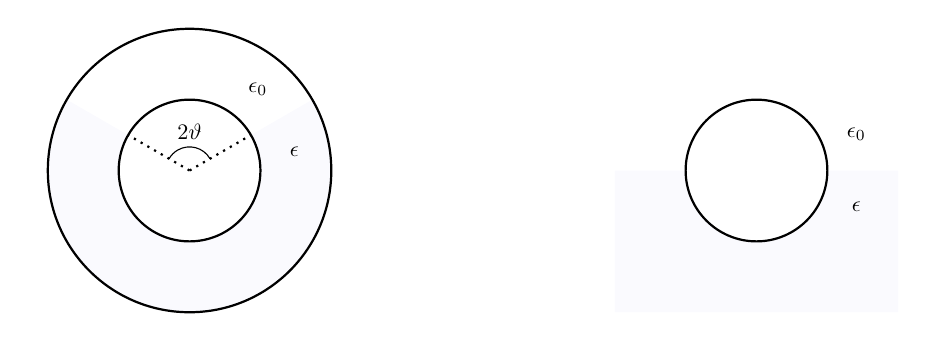
\begin{tikzpicture}[scale=0.6,every node/.style={scale=0.8}]
                \def\a{1.5}
                \def\b{3}
                \def\t{30}
                \path[fill=Lavender!20] +({180 - \t}:\b) arc[start angle={180-\t}, end angle={360+\t}, radius=\b]  -- ({\a*cos(\t)}, {\a*sin(\t)}) arc[start angle={360+\t}, end angle={180 - \t}, radius=\a] -- cycle;
                \draw[thick] (0,0) circle (\b);
                \draw[thick] (0,0) circle (\a);

                \node at +({\t + 20}:{(\a + \b)/2}) {$\epsilon_0$};
                \node at +({\t-20}:{(\a + \b)/2}) {$\epsilon$};
                \draw[thick, dotted] (0,0) -- +(\t:\a);
                \draw[thick, dotted] (0,0) -- +({180-\t}:\a);

                \draw +(\t:{\a/3}) arc[start angle={\t},end angle={180-\t},radius={\a/3}] node[midway, above] {\(2\vartheta\)};

                \begin{scope}[xshift=12cm]

                    \path[fill=Lavender!20] (-\a,0) -- (-\b,0) -- (-\b, -\b) -- (\b,-\b) -- ({\b}, 0) -- (\a, 0) arc[start angle=360, end angle=180, radius=\a] -- cycle;
                    \draw[thick] (0,0) circle (\a);

                    \node at +(20:{(\a + \b)/2}) {$\epsilon_0$};
                    \node at +(-20:{(\a + \b)/2}) {$\epsilon$};
                \end{scope}
            \end{tikzpicture}
        \end{center}
\end{exercício}
\begin{proof}[Resolução]
    Como as cascas esféricas estão mantidas a potenciais constantes, temos \(\phi(\vetor{\x}) = 0\) sempre que \(\norm{\vetor{\x}} > b\) e temos \(\phi(\vetor{\x}) = \phi_0\) sempre que \(\norm{\vetor{\x}} < a\). Alinhando o eixo \(z\) com o eixo de simetria de modo que a região \(\theta \in (\frac{\pi}{2}, \pi]\) seja a preenchida com o dielétrico linear, vemos que o problema apresenta simetria azimutal. Dessa forma, podemos escrever
    \begin{equation*}
        \phi(r \vetor{e}_r) = \begin{cases}
            0,&\text{se }r \geq b\\
            \sum_{\ell = 0}^\infty \left(A_\ell r^\ell + \frac{B_\ell}{r^{\ell + 1}}\right)P_\ell(\cos\theta),&\text{se }r \in (a,b)\text{ e }\theta \in [0, \frac{\pi}{2})\\
            \sum_{\ell = 0}^\infty \left(\alpha_\ell r^\ell + \frac{\beta_\ell}{r^{\ell + 1}}\right)P_\ell(\cos\theta),&\text{se }r \in (a,b)\text{ e }\theta \in (\frac{\pi}{2},\pi]\\
            \phi_0,&\text{se }r \leq a
        \end{cases}
    \end{equation*}
    e vemos por continuidade em \(r = a\) e \(r = b\) que
    \begin{align*}
        A_\ell b^\ell + \frac{B_\ell}{b^{\ell + 1}} = 0 \quad\text{e}\quad A_\ell a^\ell + \frac{B_\ell}{a^{\ell + 1}} = \phi_0 \delta_{\ell 0}
        &\implies B_\ell = -A_\ell b^{2\ell + 1} \quad\text{e}\quad A_\ell\left(a^\ell - \frac{b^{2\ell + 1}}{a^{\ell + 1}}\right) = \phi_0 \delta_{\ell 0}\\
        &\implies A_\ell = -\frac{a}{b - a} \phi_0 \delta_{\ell 0} \quad\text{e}\quad B_\ell = \frac{ab}{b - a} \phi_0 \delta_{\ell 0}
    \end{align*}
    para todo \(\ell \in \mathbb{N}_0\). Mutatis mutandi obtemos \(\alpha_\ell\) e \(\beta_\ell\), e concluímos que \(\alpha_\ell = A_\ell\) e \(\beta_\ell = B_\ell\)
    e que
    \begin{equation*}
        \phi(r \vetor{e}_r) = \begin{cases}
            0,&\text{se }r \geq b\\
            \frac{a\phi_0}{b - a}\left(\frac{b}{r} - 1\right),&\text{se }r \in (a,b)\\
            \phi_0,&\text{se }r \leq a
        \end{cases}
    \end{equation*}
    é o potencial em todo o espaço.
\end{proof}
